\documentclass{article}
\usepackage[a4paper, top=2cm, bottom=2cm]{geometry}

\usepackage{amsmath}
\usepackage[hidelinks]{hyperref}
%\usepackage{hyperref}
\usepackage{lastpage}  % ``n of m'' page numbering
\usepackage{enumitem}
\usepackage{graphicx}
\usepackage{float}
\usepackage{xcolor}
\newcommand{\textlightgray}[1]{\textcolor{lightgray}{#1}}
\usepackage{setspace}  % tight changelog

% Heading
\usepackage{fancyhdr}
\pagestyle{fancy}
\fancyhf{}
\lhead{\textbf{Jacky Kung}\\jwek2@cam.ac.uk}
\rhead{\textbf{How It Works}\\ \href{https://stpaulswalk-jswz.servehttp.com}{https://stpaulswalk-jswz.servehttp.com}}
\setlength{\headheight}{22.6pt}
\cfoot{Page \thepage\ of \pageref{LastPage}}
\renewcommand{\headrulewidth}{0.5pt}
\renewcommand{\footrulewidth}{0.5pt}

% Layout
\setlength{\parindent}{0em}
\addtolength{\parskip}{1ex}

% Chinese support
\usepackage{CJKutf8}
\newcommand{\chinese}[1]{\begin{CJK}{UTF8}{bsmi}#1\end{CJK}}

\setcounter{section}{-1}

\begin{document}

\section*{Foreword}

I'm writing this article, in part to share what I've learnt about HTTPS, and also in part to remind the future me about the nitty-gritty that I'll likely forget in one year's time. An attempt was made in simplifying certain details. I'll link resources at the end for further exploration. May this article serve as a gentle introduction to anyone unfamiliar with but interested in HTTPS!

\emph{If there are parts that are unclear, please do reach out to me at the email address on the top left. I look forward to hearing your feedback!}

\tableofcontents

\newpage
\section{Changelog}
{\setstretch{0}

\textbf{v1 (1 Oct 2022)}
\begin{itemize}
    \item Initial version.
\end{itemize}

%\textbf{v2 (DATE)}
%\begin{itemize}
%    \item
%\end{itemize}
}

\newpage
\section{Abstract Idea of this Web Application}
Every website is just a pretty user interface to a database (a huge excel sheet, of sorts). For this website, the database holds our electricity readings, and sits on "Jacky's device", which happens to be a Raspberry Pi machine. It's connected to the power socket somewhere, and as long as it is powered, this website can be reached.

This is the general idea:

\begin{figure}[H]
    \centering
    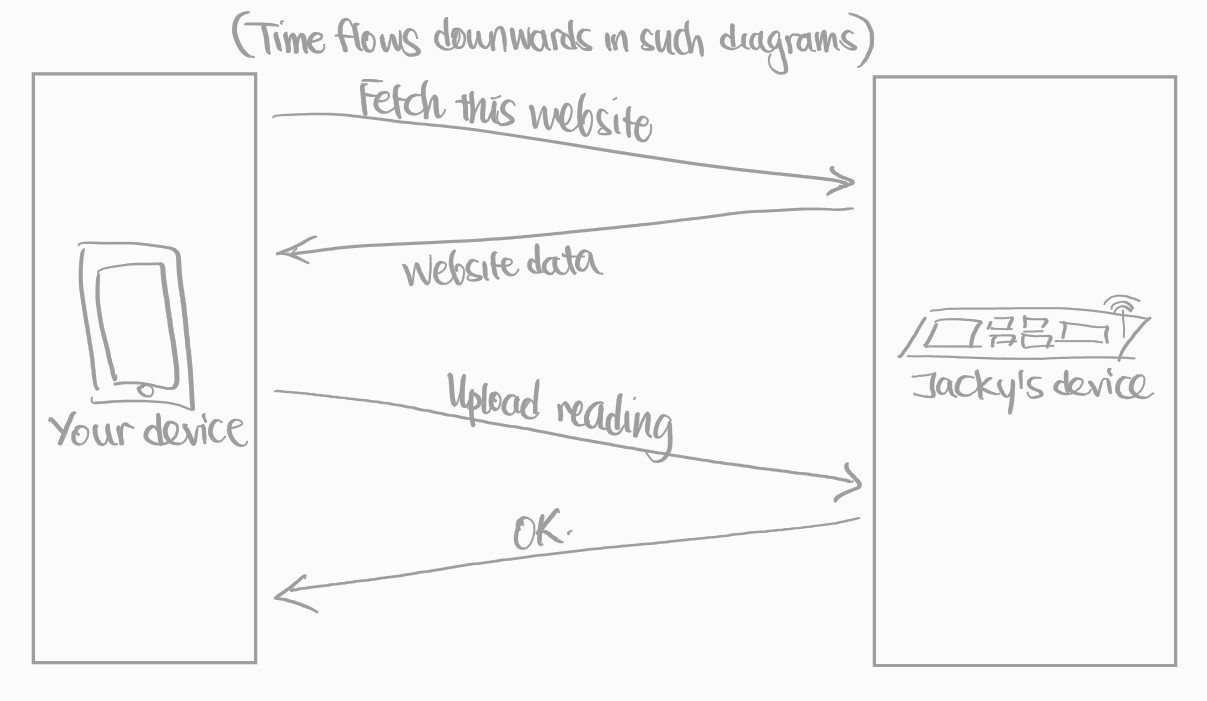
\includegraphics{Chapter 0 General Request Flow.png}
    \caption{The arrows signify the passing of messages, in an abstract sense. How this concretely happens will be discussed in moderate detail later in this article.}
\end{figure}

But how do we ensure that information flows between your device and Jacky's device safely? I.e. we don't want third parties to peak into our messages, modify them, or re-route your connection such that you're actually talking to some \chinese{隔壁老王}'s device instead of Jacky's device. These are all prevented by HTTPS, and this article goes into moderate depth about how it all works.

\newpage
\section{Communicating over the Internet}
\subsection{Internet infrastructure}

Every computing device in the world is assigned a unique \textbf{public IP address}. It's like a postal code for the Internet. In conversations that happen across the Internet (transmission of data), messages all contain a \emph{source IP address} and a \emph{destination IP address}.

There's also a concept of \textbf{ports}. Using the snail-mail analogy, a port is like a front door of the device, through which messages are sent and received. Each device has 65536 ports, and each conversation (e.g. web browser visiting this website) occupies one port, generally speaking. This allows a device to have up to 65536 independent conversations. All messages thus also contain a \emph{source port} and a \emph{destination port}.

\begin{figure}[H]
    \centering
    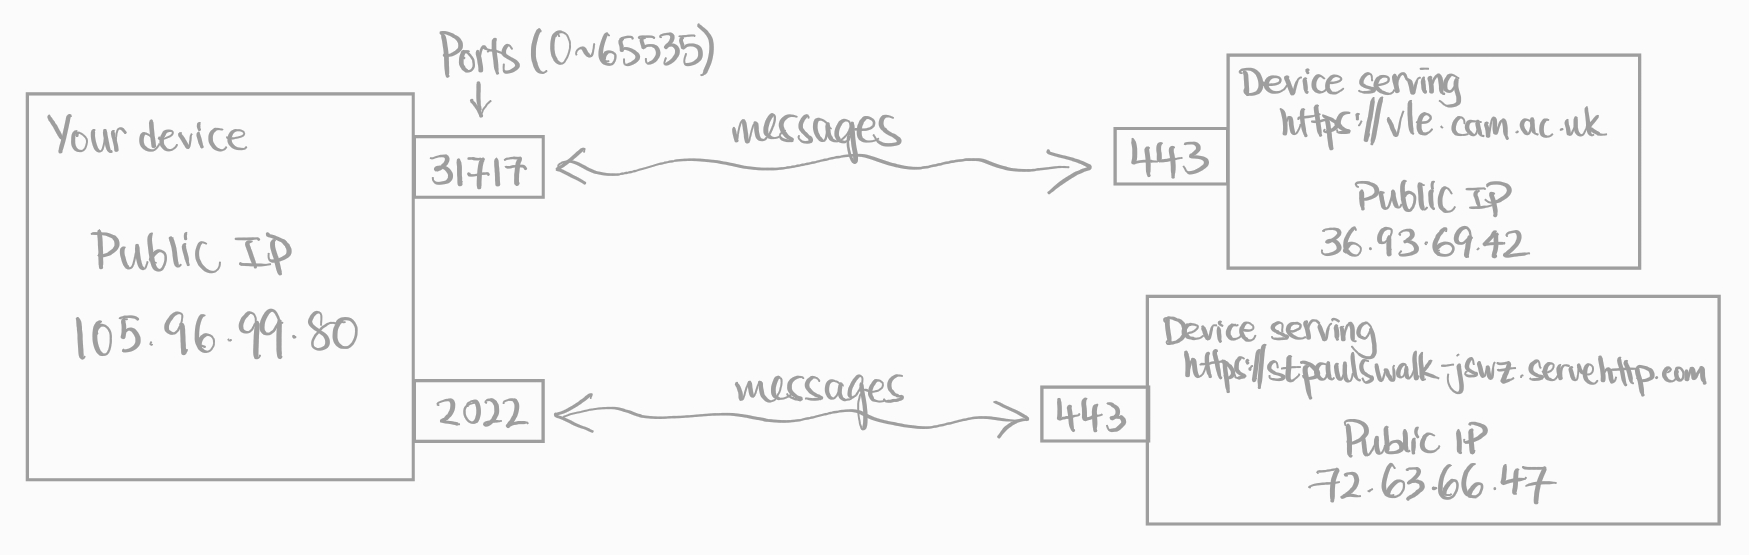
\includegraphics{Chapter 1 IP Arch.png}
    \caption{The arrows signify the passing of messages, in an abstract sense. How this concretely happens will be discussed in moderate detail later in this article.}
\end{figure}

If you're visiting a HTTPS website, the destination port is always 443 (Internet convention).

Actually, the first sentence of this section is a white lie. See \S\ref{nat}, which talks about \textbf{local IP addresses} (the counterpart to public IP addresses).

\subsection{Domain Name Service (DNS)}
Since all messages have source and destination IP addresses, to talk to Jacky's device, who is providing this website and its data, you'll need send requests to its IP address.

But we don't usually enter IP addresses into our browser's address bar (though we certainly can). The key concept here is: every URL is an alias to an underlying IP address\footnote{Ignoring larger services like Google which actually have more than 1 IP address backing the website \texttt{https://www.google.com} for fault tolerance reasons.}. When you type \verb|https://stpaulswalk-jswz.servehttp.com| into your address bar, your browser performs a process called \textbf{DNS Lookup} to find out its underlying IP address.

\begin{figure}[H]
    \centering
    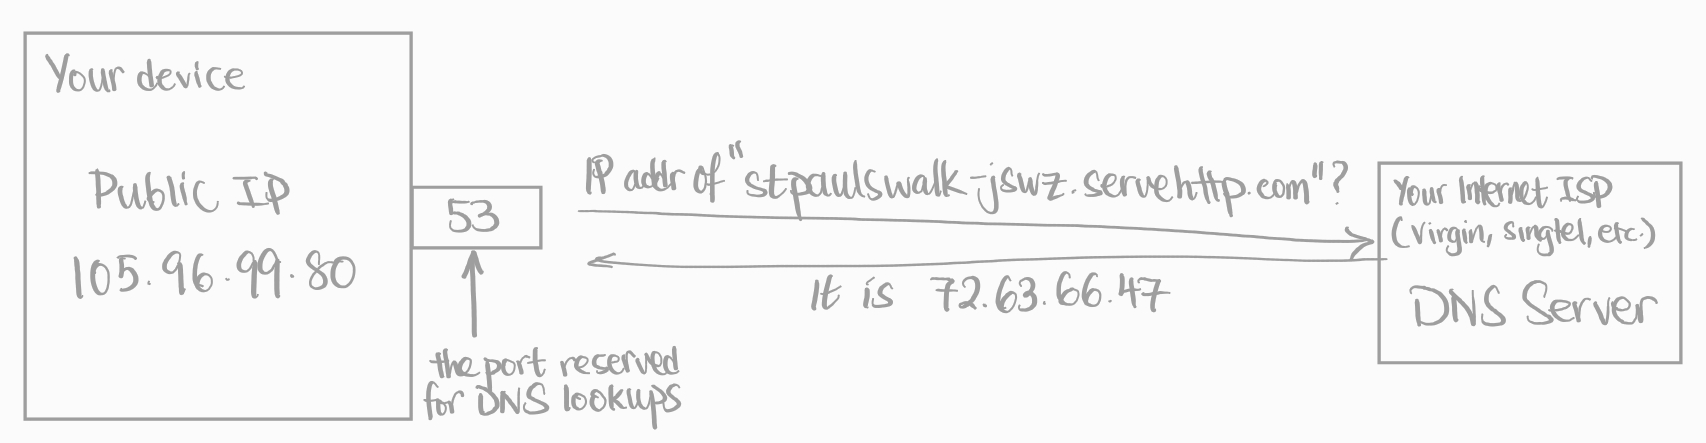
\includegraphics{Chapter 1 DNS.png}
    \caption{DNS Lookup.}
\end{figure}

Now you can reach Jacky's device via its IP address.

\subsection{Public/Local IP addresses and Network Address Translation (NAT)}
\label{nat}

Here's a caveat on IP addresses: they range from \verb|0.0.0.0| to \verb|255.255.255.255|. This gives us $256^4 = 4\ 294\ 967\ 296$ unique IP addresses. If all of them were \emph{public IP addresses} used to uniquely identify every device on Earth, we'd have already run out of them many years ago!

The Internet infrastructure engineers thought of a solution: instead of treating all IP addresses equally as public IP addresses, we give different subsets of addresses different roles:
\begin{itemize}
    \item \textbf{Public IP addresses} are used to identify a group of machines, typically all those connected to a single Home/Office WiFi router.
    \item \textbf{Local IP addresses} are used to identify each machine within the context of some\\ Home/Office WiFi router. These either look like:
    \begin{itemize}
        \item \verb|192.168.x.x|,
        \item \verb|172.[16 to 31].x.x|, or
        \item \verb|10.x.x.x|
    \end{itemize}
    This list is exhaustive.

    For instance, an address like \verb|192.168.1.1| does not uniquely identify a device in the world, but does uniquely identify a device among those connected to a Home/Office WiFi router.
\end{itemize}

\begin{figure}[H]
    \centering
    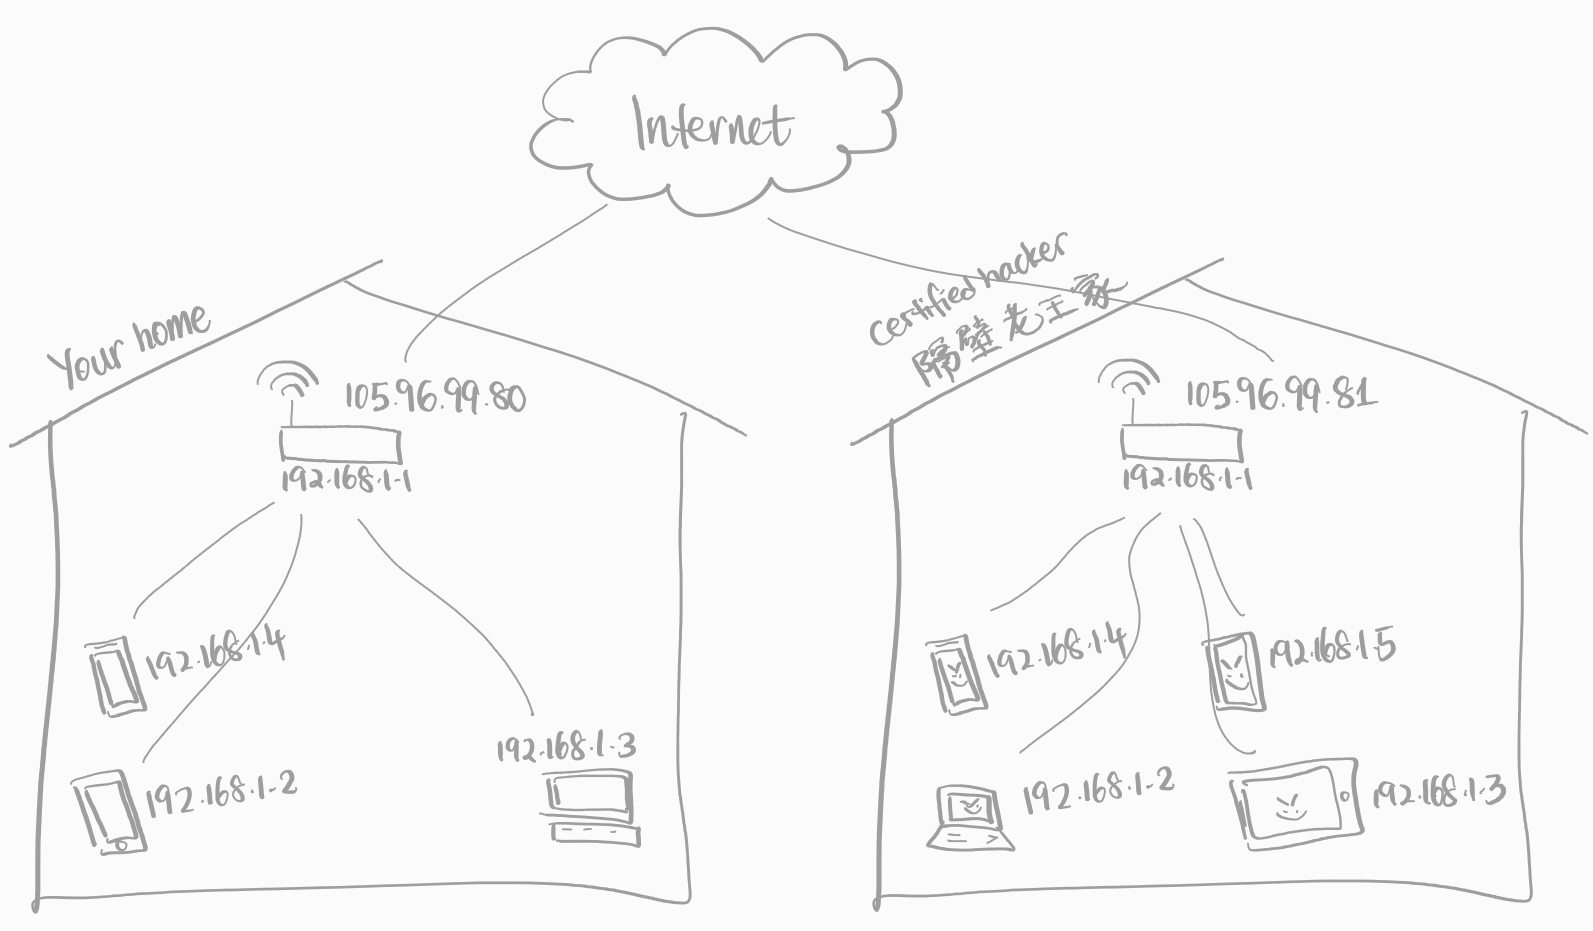
\includegraphics{Chapter 1 Public Local IP.png}
    \caption{Public VS Local IP Addresses. Those starting with \texttt{192.168.x.x} are local IP addresses. The WiFi router's local IP address is \texttt{192.168.1.1}, and this is a common default. Try typing this into your browser's address bar: you should arrive at your WiFi router's settings page!}
\end{figure}

Notice how every time your messages pass through a router, the message's source and destination IP address and ports have to change:
\begin{itemize}
    \item Between public IP address and local IP address
    \item Between public port and local port
\end{itemize}
This conversion is called \textbf{Network Address Translation (NAT)}.

\begin{figure}[H]
    \centering
    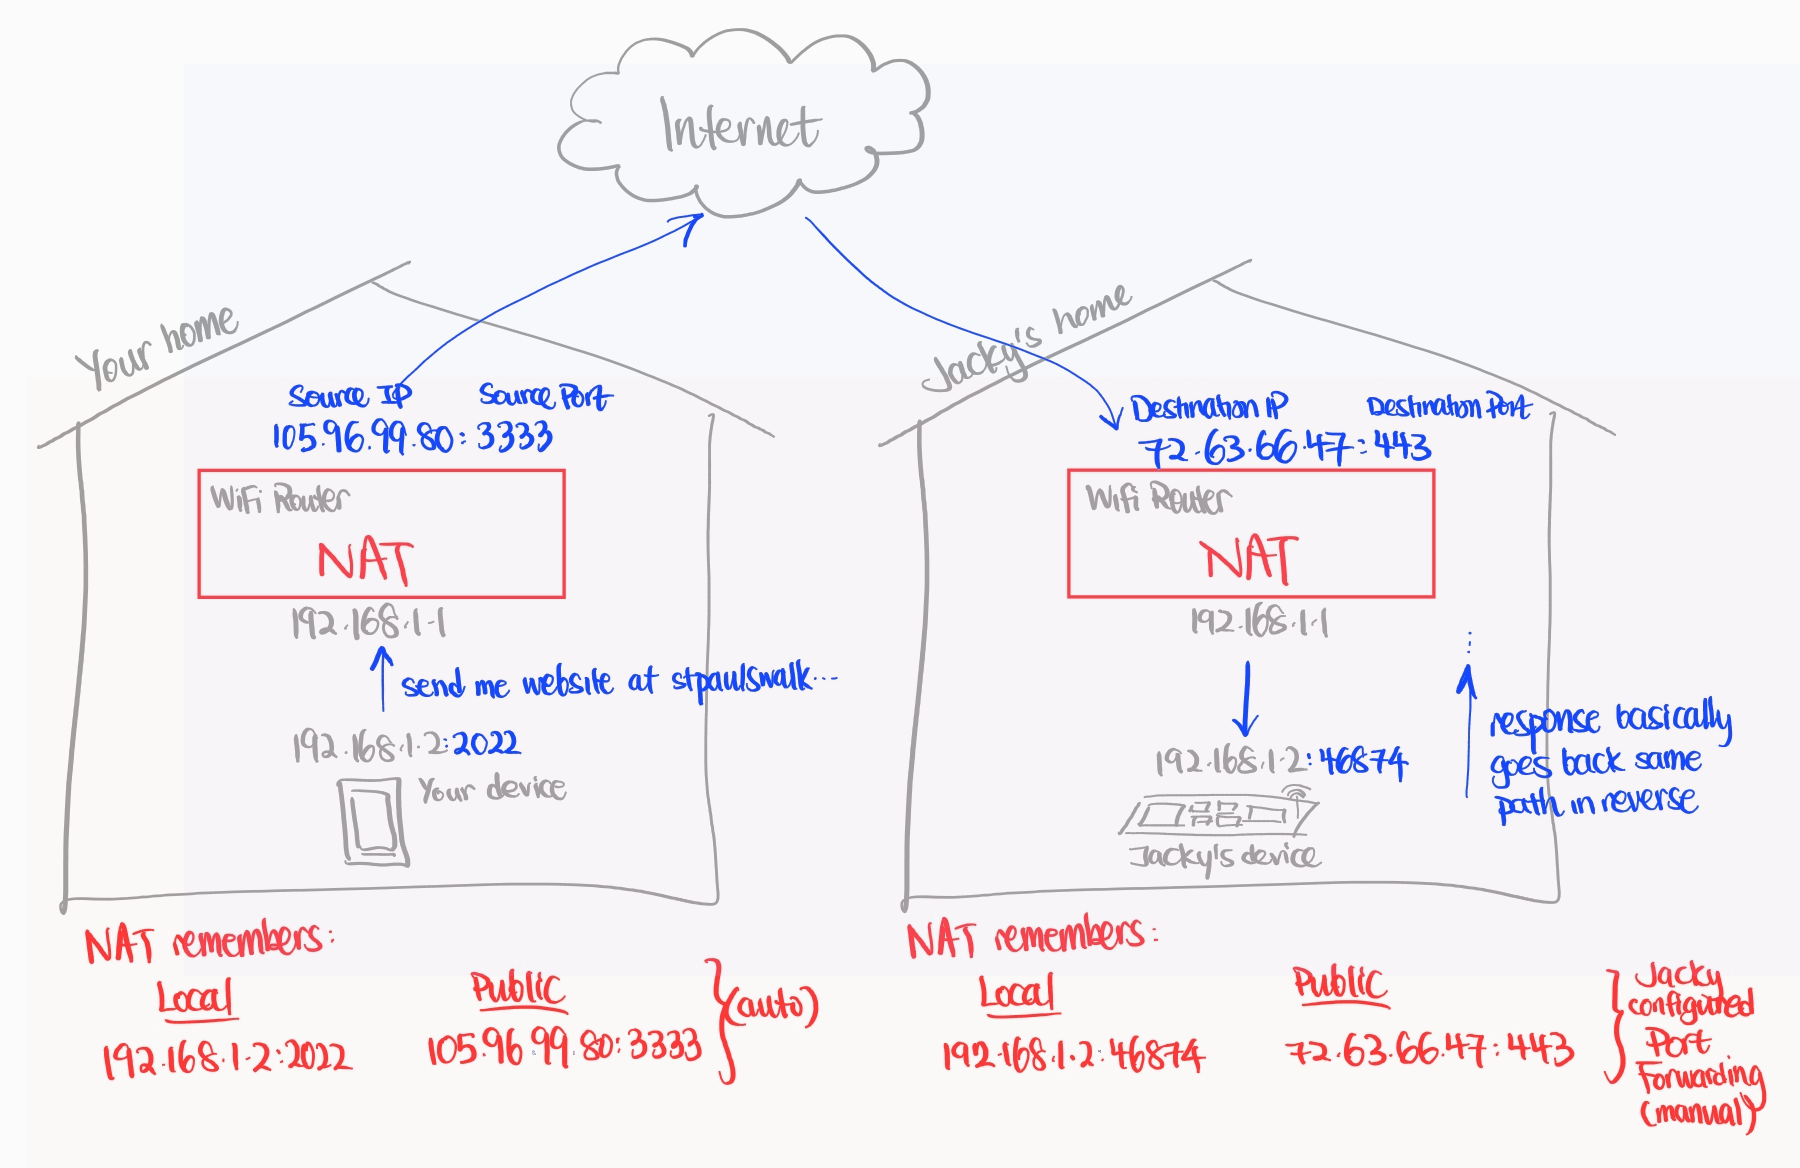
\includegraphics{Chapter 1 Public Local IP Full.png}
    \caption{Process of making a request from your device to Jacky's device. The notation \texttt{192.168.1.2:2022} represents port \texttt{2022} on the device with IP address \texttt{192.168.1.2}.}
    \label{fig:ipfull}
\end{figure}

With reference to Figure \ref{fig:ipfull}, as your device's message makes it through your WiFi router, the message will be modified by process of Network Address Translation:
\begin{itemize}
    \item Source IP address from \verb|192.168.1.2| (local) to \verb|105.96.99.80| (public)
    \item Source port from \verb|2022| (local) to \verb|3333| (public)
\end{itemize}

Similar translation happens at Jacky's WiFi router, from public stuffs to local stuffs.

Where is NAT conducted? Not everywhere! It typically only happens at the Home/Office WiFi routers that connect your home/office's devices to the wider Internet. Your router is doing some pretty important work under the hood!

\subsubsection{Port Forwarding}
NAT happens automatically if you're not a server serving data/websites, as for the case of your WiFi router in Figure \ref{fig:ipfull}.

For the case of Jacky's device, who is serving a HTTPS website, Jacky needs to manually configure his router to pass all HTTPS requests coming in from the Internet to his device. This is called \textbf{Port Forwarding}: manually configuring the WiFi router's admin settings, to translate between \verb|72.63.66.47:443| and \verb|192.168.1.2:46874| (using numbers from Figure \ref{fig:ipfull}).

This concludes the Communicating Over the Internet section. You now know the details of how your device communicates with Jacky's device.

\newpage
\section{Server Authenticity}
\^{} For the rest of this article, I make claims about having ``100\% certainty''. This guarantee relies on the assumption that prime factorisation is very slow for computers. Much of our cyber security relies on this assumption. (Saying that this is an understatement is an understatement itself: the details are some R21 Computer Science gore that I won't elaborate on.)


%> Hardest chapter to write and digest.
%> Jacky's machine proves to you that you are talking to Jacky's machine
%
\subsection{Theory: What does HTTPS achieve?}
\label{theory}
In short, establish trust between the two communicating parties (e.g. your device and Jacky's device). Trust is established using three core concepts:

\begin{enumerate}[label=\arabic*.]
    \item \textbf{Authenticity}\\ This means proving (yes, with 100\%\^{} certainty) that you are who you claim to be. Both server and client must authenticate themselves to one another: this is how you trust that whoever sending you this website's data is indeed Jacky's device, and how Jacky's device knows that you are the one sending them data requests and new electricity readings.
    \item \textbf{Integrity}\\ This means proving (yes, with 100\%\^{} certainty) that a message hasn't been tampered by a third party while in transit.
    \item \textbf{Encryption}\\ This is what most people think of when hearing HTTPS vs HTTP. We don't want anybody to be able to read data you're receiving/sending while it's in transit.
\end{enumerate}
Why are these important? Consider what happens when any of them are taken away.
\begin{itemize}
    \item Take away authenticity while keeping encryption and integrity. Although no third party can read or modify your messages, you cannot trust who you're talking to. You might be receiving this website and data from \chinese{隔壁老王}'s device instead of Jacky's device. Can you really trust who you're receiving data from?
    \item Take away integrity while keeping encryption and authenticity. Although no third party can read your messages, and you trust who you are talking to, a third party may have intercepted and modified messages while they're in transit. \chinese{隔壁老王} may have injected his version of the website in place of what Jacky's device intended to send. Can you really trust what you're receiving?
    \item Take away encryption while keeping authenticity and integrity. Although you trust who you are talking to, and that no third party modified your messages, now third parties can read your messages. Your sensitive personal information like your name and email address, transmitted by Jacky's device, might be inspected by \chinese{隔壁老王} eavesdropping on incoming Internet signals (yes, that's possible). Can you trust that sensitive data hasn't been leaked to a third party?
\end{itemize}

\subsubsection{Green padlock next to browser's address bar}
When the green padlock is present for a website, \emph{all} 3 of the properties in \S\ref{theory} are satisfied. Thus you can be 100\%\^{} sure that you're talking to the right person, and that nobody is able to read or modify your in-transit messages.

\subsection{How HTTPS achieves authenticity, integrity and encryption}
\begin{itemize}
    \item Authenticity: \textbf{HTTPS Certificate}
    \item Integrity: \textbf{HTTPS Signature}
    \item Encryption: Cryptography. In particular, symmetric encryption.
\end{itemize}

When you visit \verb|https://stpaulswalk-jswz.servehttp.com|, you first make a HTTPS connection to Jacky's device. Even before Jacky's device sends back website data, the two devices engage in a \textbf{HTTPS handshake}, to establish the 3 properties in \S\ref{theory}. Only after these 3 are obtained successfully, will Jacky's device send you website data.

%<!--
%How does Jacky's device make you trust that you're talking to it, and not 隔壁老王? Via both HTTPS Certificate and HTTPS Signature. Both authentication and integrity are necessary for this trust! -->

\subsection{Interlude: Public Key Cryptography}
\emph{(Don't be intimidated by the mathematical expressions from here on! I use them to save space: the same idea will take a paragraph of words to describe, but just one line of equation.)}

Here's what we need to know about cryptography. Take it on faith that its mathematically very, very difficult to crack these systems; we can treat it as effectively 100\%\^{} effective.

In public key cryptography, devices that wish to prove authenticity of their messages (like Jacky's device) each generate a public-private \textbf{key pair}. The private key is kept strictly secret by the device's owner. The public key is distributed for the world to see and use.

\subsubsection{Notation}
I'll use the notation $PBK_X$ to denote $X$'s public key, and $PVK_X$ to denote $X$'s private key.

I'll use the notation $\text{encrypt}_K\left(\text{data}\right)$ to denote the outcome of encrypting $\text{data}$ using the key $K$. The key may be private or public, depending on the situation.

\subsubsection{Important Properties}
\begin{itemize}
    \item $$\text{decrypt}_{PVK_X}\left(\text{encrypt}_{PBK_X}\left(\text{data}\right)\right) = \text{data}$$
%
%    In particular, if some data has been encrypted with a public key, we must use the private key to decrypt it: \emph{only} the private key can decrypt it.
    \item \begin{equation}
        \text{decrypt}_{PBK_X}\left(\text{encrypt}_{PVK_X}\left(\text{data}\right)\right) = \text{data} \label{keyeqn}
    \end{equation}

    In particular, if some data can be decrypted by a public key (i.e. after decryption we don't get garbage), it means the private key must've been used to encrypt it. %We can make this deduction because the private key $PVK_X$ is known only by the device that generated it $X$. This is the crux to all this working.
\end{itemize}

Any more detail is information overload so I'll skip them. The basic principles relevant to us are:
\begin{itemize}
    \item If you use one key to encrypt something, the other key in the key pair must be used to decrypt it.

    Lose either key in the key pair, and your encrypted messages will become lost as encrypted garbage forever.
    \item One of the keys in the key pair must be kept secret (only known by the party who generated it). The other one may be public knowledge.

    Exposing private keys to the public immediately breaks down the security guarantees that public key cryptography gives us. They must be kept absolutely secret.
\end{itemize}

\subsection{The HTTPS Handshake}
How the 3 desired properties in \S\ref{theory} is achieved is best illustrated with some concrete details.

Before we move on, here's some context:
\begin{itemize}
    \item \emph{NoIP} is the service Jacky is using to reserve the URL \verb|stpaulswalk-jswz.servehttp.com|. It's free and it basically allows DNS lookups (by your device) to translate this URL to Jacky's device's public IP address. Their website can be found \href{https://www.noip.com/}{here}.
    \item \emph{TrustCor} is a \textbf{Certificate Authority}. Certificate Authorities provide HTTPS certificates to hosts of websites.
\end{itemize}

HTTPS Certificates are simply a bunch of information signed (encrypted) using a Certificate Authority's private key $PVK_{CA}$ (I'll use $PVK_{CA}$ to refer to \emph{TrustCor}'s private key in this article, since it's the only Certificate Authority I'll talk about).

Why is this signing important? This is elaborated in the next section.

\subsubsection{Establishing trust via Delegation of Trust}
% Think of all traffic your device receives from the Internet as having an unknown sender: they're ultimately all 0s and 1s, and anyone can change them while they're in transit. An incoming message that says "Trust me, I'm for sure sent from Jacky's device" is omega sus.

HTTPS achieves authenticity via what I call ``delegation of trust'':
\begin{itemize}
    \item Your device unquestioningly trusts a list of \textbf{Certificate Authorities (CAs)}\footnote{Actually, your device trusts a list of \emph{Root} CAs. There is a hierarchy of CAs; the one up on top are Root CAs. This detail isn't necessary for understanding this article.}. You may add or remove CAs from this list via your device's security settings.
    \item Whoever these CAs trust, your device also trusts, unquestioningly, by delegation of trust.
    \item These CAs are trusted (by many devices like yours) to only hand out HTTPS certificates to people like Jacky after the CA has done their due diligence (performed checks).

    What checks? That Jacky has ownership over the URL that he's requesting a HTTPS Certificate for.
\end{itemize}

The certificate authority that Jacky's device uses is \emph{TrustCor}. \emph{TrustCor} (and any other CA), needs to verify that Jacky is indeed the owner of and has control over \verb|https://stpaulswalk-jswz.servehttp.com|.

\subsubsection{Before the HTTPS Handshake}
Here is what happens before the handshake:

\begin{figure}[H]
    \centering
    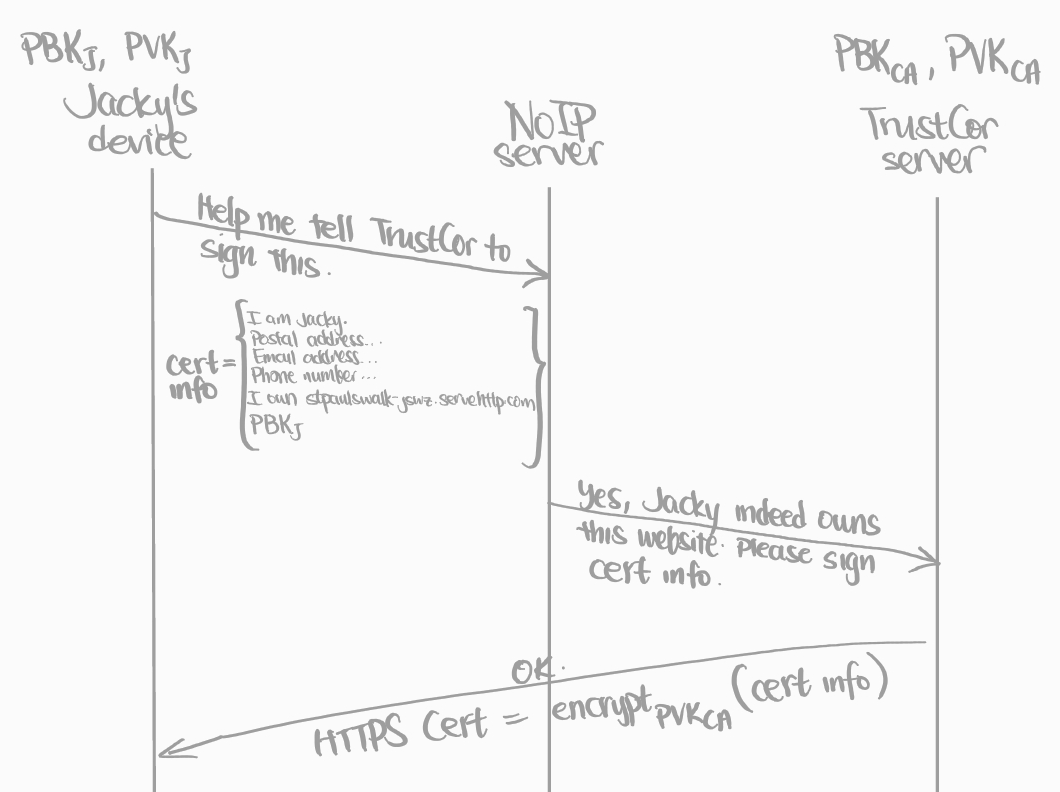
\includegraphics{Chapter 2 Pre Handshake.png}
    \caption{The process of \textbf{Certificate Signing Request (CSR)}, where Jacky asks \emph{TrustCor} to sign a bunch of certificate information.}
\end{figure}

\begin{itemize}
    \item Jacky sends a set of information ($\text{cert info}$) to \emph{NoIP}, requesting for a HTTPS certificate signed by \emph{TrustCor} for \verb|stpaulswalk-jswz.servehttp.com|. \emph{NoIP} forwards this request to \emph{TrustCor}, additionally confirming that Jacky indeed owns the URL\\ \verb|stpaulswalk-jswz.servehttp.com|.
    \item \emph{TrustCor} has its own key pair: $PBK_{CA}$ (public key) and $PVK_{CA}$ (private key).
    \item \emph{TrustCor} signs ($\text{cert info}$) and sends the HTTPS certificate to Jacky:
    $$\underbrace{\text{encrypt}_{PVK_{CA}}\left(\text{cert info}\right)}_{\text{HTTPS Cert}}$$
\end{itemize}
\newpage

\subsubsection{During the HTTPS Handshake}
This is what happens during the handshake:

\begin{figure}[H]
    \centering
    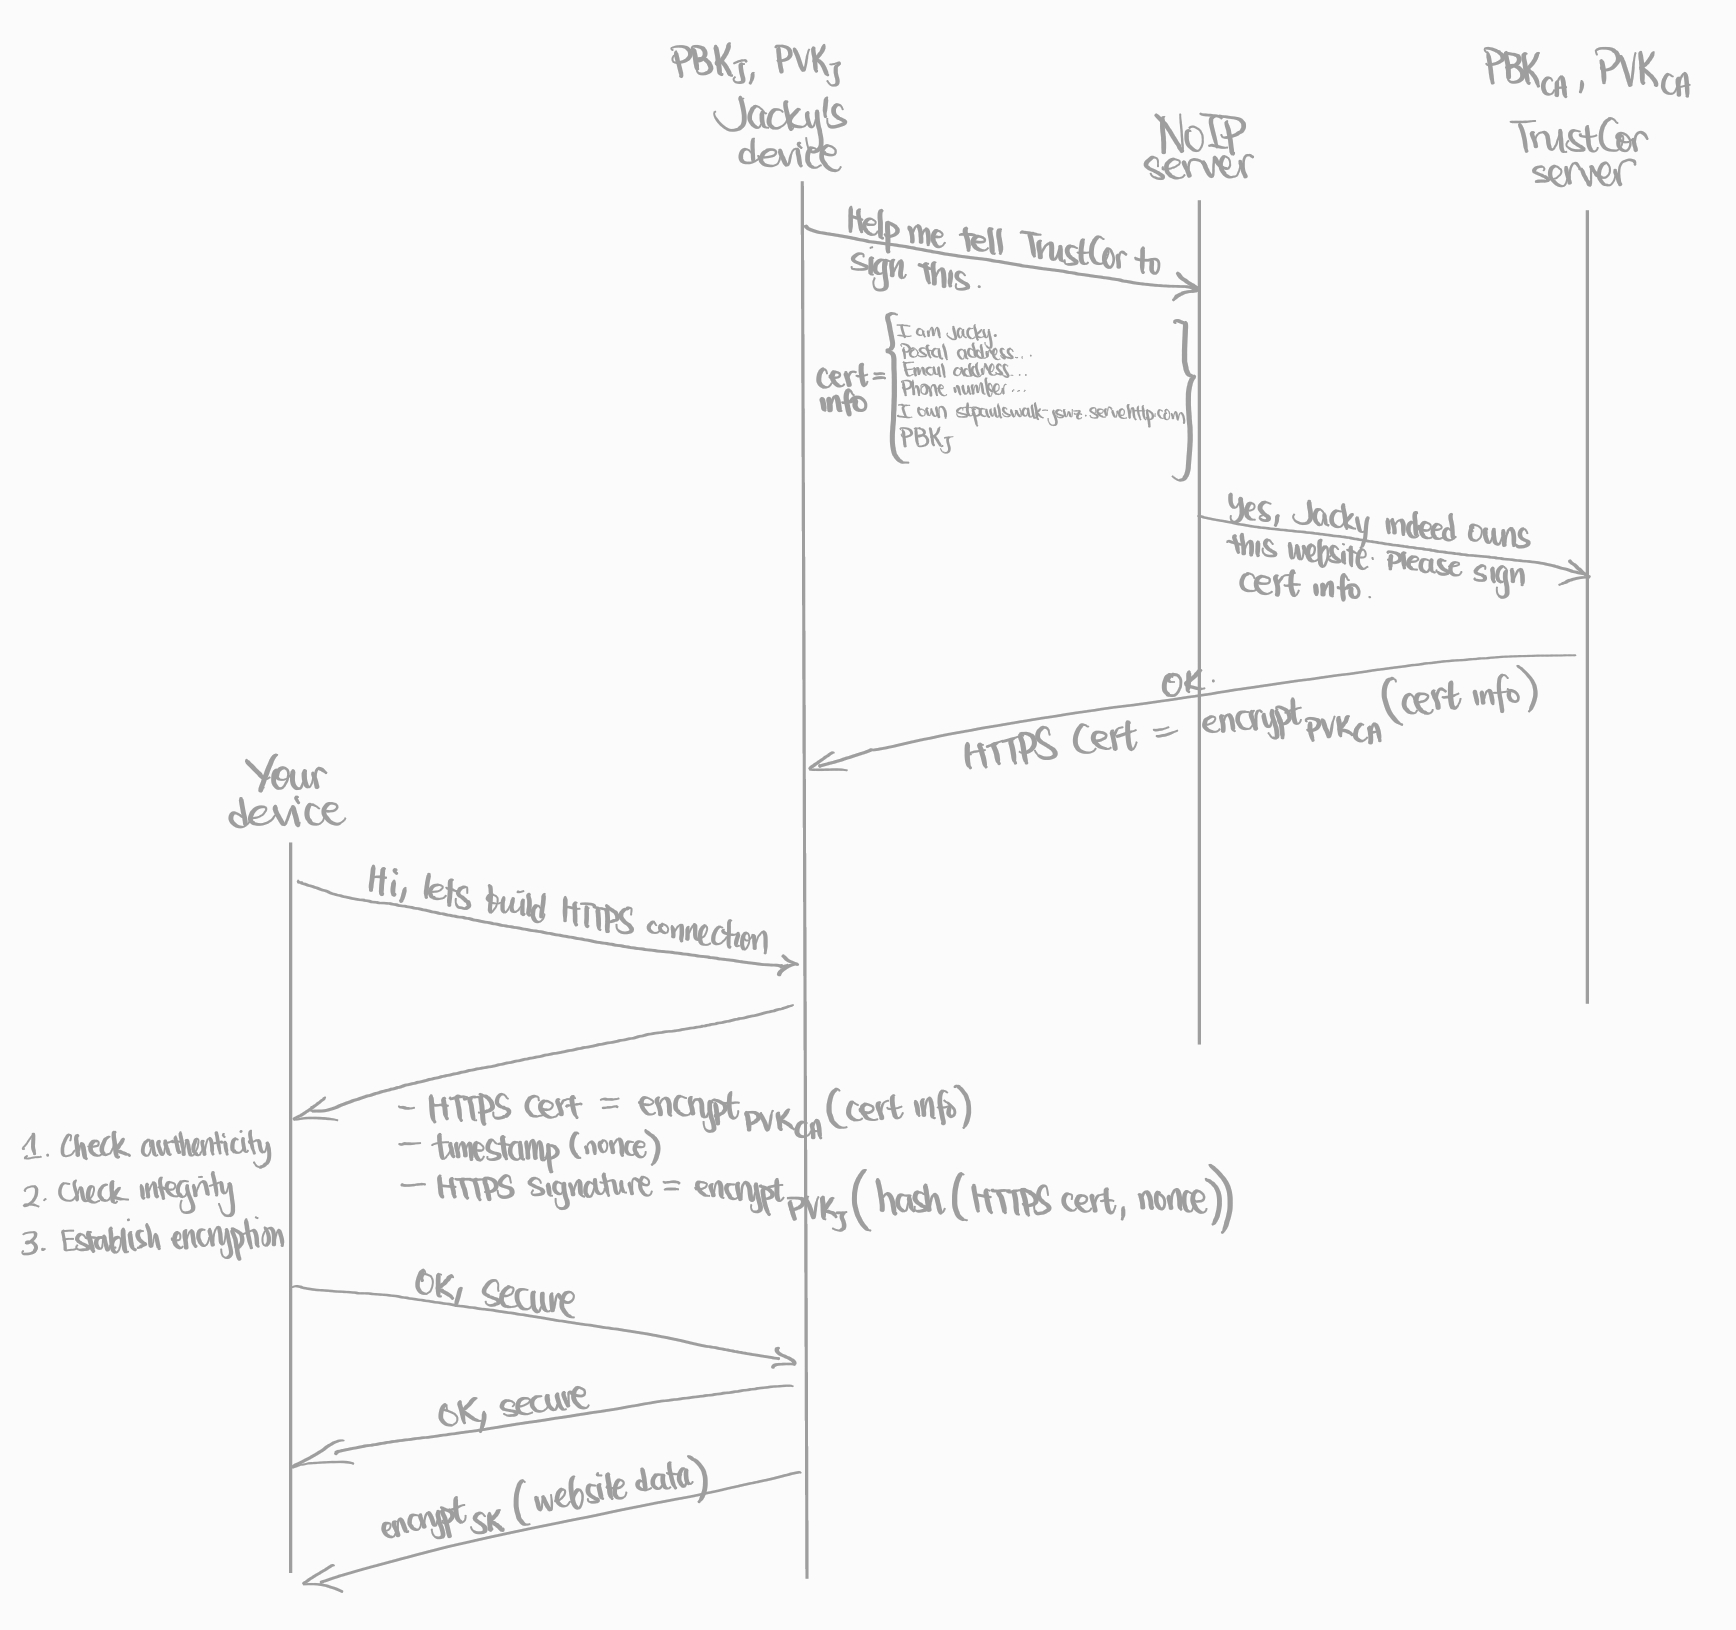
\includegraphics{Chapter 2 Handshake.png}
    \caption{Top right: Certificate Signing Request (CSR). Bottom left: HTTPS Handshake. $SK$ refers to Session Key, which is explained near the end of this section.}
\end{figure}

\begin{itemize}
    \item Your device makes a request to Jacky's device.
    \item Jacky's device sends back 3 things as part of the handshake:
    \begin{itemize}
        \item $\underbrace{\text{encrypt}_{PVK_{CA}}\left(\text{cert info}\right)}_{\text{HTTPS Certificate}}$
        \item a nonce (to prevent replay attacks)
        \item $\underbrace{\text{encrypt}_{PVK_J}\left(\text{hash}\left(\underbrace{\text{encrypt}_{PVK_{CA}}\left(\text{cert info}\right)}_{\text{HTTPS Certificate}}, \text{nonce}\right)\right)}_{\text{HTTPS Signature}}$
    \end{itemize}
\end{itemize}

\newpage
\subsubsection{During the HTTPS Handshake: Checks done by your device}
Now, your device performs checks to achieve the 3 desired properties in \S\ref{theory}:
\begin{enumerate}[label=\arabic*.]
    \item \textbf{Authenticity}: did this message really come from Jacky's device, and not \chinese{隔壁老王}'s device?
    \begin{enumerate}[label=1.\arabic*.]
        \item Your device unquestioningly trusts \emph{TrustCor}. Thus, \emph{TrustCor}'s public key is stored in your device's security settings. Your device thus obtains $PBK_{CA}$ this way.
        \item Your device decrypts the HTTPS certificate using $PBK_{CA}$:
        $$\text{decrypt}_{PBK_{CA}}\left(\underbrace{\text{encrypt}_{PVK_{CA}}\left(\text{cert info}\right)}_{\text{HTTPS Certificate}}\right)$$
        If the result is not unreadable garbage (i.e. it is ($\text{cert info}$)), then by important property \eqref{keyeqn}, we are 100\%\^{} sure that \emph{TrustCor} is the one who issued this HTTPS certificate.

        Thus, we know that \emph{TrustCor} trusts Jacky and Jacky's device, to be who they claim they are (\emph{NoIP} helped by verifying that Jacky owns the website \verb|stpaulswalk-jswz.servehttp.com| served by Jacky's device).

        By delegation of trust, your device also trusts Jacky's device. Thus, we have achieved \textbf{authenticity} of the server.
    \end{enumerate}
    \item \textbf{Integrity}: did this message arrive untampered?
    \begin{enumerate}[label=2.\arabic*.]
        \item Your device hashes the first two things that Jacky's device sent back:
        $$\text{hash}\left(\underbrace{\text{encrypt}_{PVK_{CA}}\left(\text{cert info}\right)}_{\text{HTTPS Certificate}}, \text{nonce}\right)$$
        \item Your device obtains $PBK_J$ from within ($\text{cert info}$), which is obtained from step 1.2 above. This is Jacky's device's public key, contained within the decrypted HTTPS Certificate, which we now know is guaranteed\^{} authentic.
        \item Your device decrypts the HTTPS Signature (third thing Jacky's device sent back) using $PBK_J$:
        $$\text{decrypt}_{PBK_J}\left(\underbrace{\text{encrypt}_{PVK_J}\left(\text{hash}\left(\underbrace{\text{encrypt}_{PVK_{CA}}\left(\text{cert info}\right)}_{\text{HTTPS Certificate}}, \text{nonce}\right)\right)}_{\text{HTTPS Signature}}\right)$$
        \item Your device checks if the values obtained in steps 1 and 3 above are the same. If they are, then we have \textbf{integrity}. Why? Because if say \chinese{隔壁老王} tampered with any of the 3 things sent by Jacky's device, this comparison will fail:
        \begin{itemize}
            \item If \chinese{隔壁老王} tampered with the HTTPS Certificate, then the values in steps 1 and 3 will not match:
            \begin{align*}
                & \text{hash}\left(\underbrace{\text{encrypt}_{PVK_{\text{\chinese{隔壁老王}}}}\left(\text{mutated}\right)}_{\text{Tampered HTTPS Certificate}}, \text{nonce}\right) \\
                & \neq \text{decrypt}_{PBK_J}\left(\underbrace{\text{encrypt}_{PVK_J}\left(\text{hash}\left(\underbrace{\text{encrypt}_{PVK_{CA}}\left(\text{cert info}\right)}_{\text{HTTPS Certificate}}, \text{nonce}\right)\right)}_{\text{HTTPS Signature}}\right) \\
                & = \text{hash}\left(\underbrace{\text{encrypt}_{PVK_{CA}}\left(\text{cert info}\right)}_{\text{HTTPS Certificate}}, \text{nonce}\right)
            \end{align*}
            \newpage
            \item If \chinese{隔壁老王} tampered with the nonce (e.g. he tried to conduct a replay attack), then again the values in steps 1 and 3 will not match:
            \begin{align*}
                & \text{hash}\left(\underbrace{\text{encrypt}_{PVK_{CA}}\left(\text{cert info}\right)}_{\text{HTTPS Certificate}}, \text{tampered nonce}\right) \\
                & \neq \text{decrypt}_{PBK_J}\left(\underbrace{\text{encrypt}_{PVK_J}\left(\text{hash}\left(\underbrace{\text{encrypt}_{PVK_{CA}}\left(\text{cert info}\right)}_{\text{HTTPS Certificate}}, \text{nonce}\right)\right)}_{\text{HTTPS Signature}}\right) \\
                & = \text{hash}\left(\underbrace{\text{encrypt}_{PVK_{CA}}\left(\text{cert info}\right)}_{\text{HTTPS Certificate}}, \text{nonce}\right)
            \end{align*}
            \item If \chinese{隔壁老王} tampered with the HTTPS Signature, then again the values in steps 1 and 3 will not match:
            \begin{align*}
                & \text{hash}\left(\underbrace{\text{encrypt}_{PVK_{CA}}\left(\text{cert info}\right)}_{\text{HTTPS Certificate}}, \text{nonce}\right) \\
                & \neq \text{decrypt}_{PBK_J}\left(\underbrace{\text{encrypt}_{PVK_{\text{\chinese{隔壁老王}}}}\left(\text{mutated}\right)}_{\text{Tampered HTTPS Signature}}\right)
            \end{align*}
        \end{itemize}
        Notice how in all three of the above, the best \chinese{隔壁老王} can do is to encrypt using his own private key $PVK_{\text{\chinese{隔壁老王}}}$ (basically any value that is extremely unlikely to be the same as $PVK_{CA}$ or $PVK_J$, since these values are kept secret by \emph{TrustCor} and Jacky respectively). Thus, keeping your own private keys secret is crucial for achieving \textbf{integrity}!
    \end{enumerate}
    \item \textbf{Encryption}: I told a white lie, again. Jacky's device actually sends back 4 things, not 3. The fourth thing sent back is a set of cryptographic parameters, used to establish a session key $SK$ used to encrypt website data after the handshake. Details are omitted; I am mostly clueless about its gory details too. \emph{(I'll learn more about it in Year 3: ask me one year later, hahaha.)}
\end{enumerate}

This concludes the Server Authenticity section. You now know how your device is able to trust data that comes from someone that claims they are Jacky's device. You now know what happens before the green padlock is shown in your browser, namely the HTTPS Handshake. In other words, we have server authenticity: you know you're talking to the genuine Jacky's device.

\newpage
\section{Client Authenticity}
Now, the reverse of Server Authenticity is also required. Jacky's device wants client authenticity: it wants to know that they're talking with the genuine \emph{you}.

This website uses \emph{Auth0} to provide users with login functionality. Assuming you don't use weak passwords or share your login credentials with others, \emph{only you} are able to login to your social accounts. By logging in (e.g. via Google sign-in), you're proving to \emph{Auth0} that the person who just triggered the log in is \emph{you}. \emph{Auth0} then passes your personal information (name and email only) to Jacky's device. This is how Jacky's device gets client authenticity.

When your device makes a request to Jacky's device, you also send along something called a \textbf{JSON Web Token (JWT)}. This is a (long) string of text that \emph{Auth0} gives to your device only after you log in via \emph{Auth0} (e.g. Google login).

Notice that without a JWT, Jacky's device refuses to respond to any requests for data.

\begin{figure}[H]
    \centering
    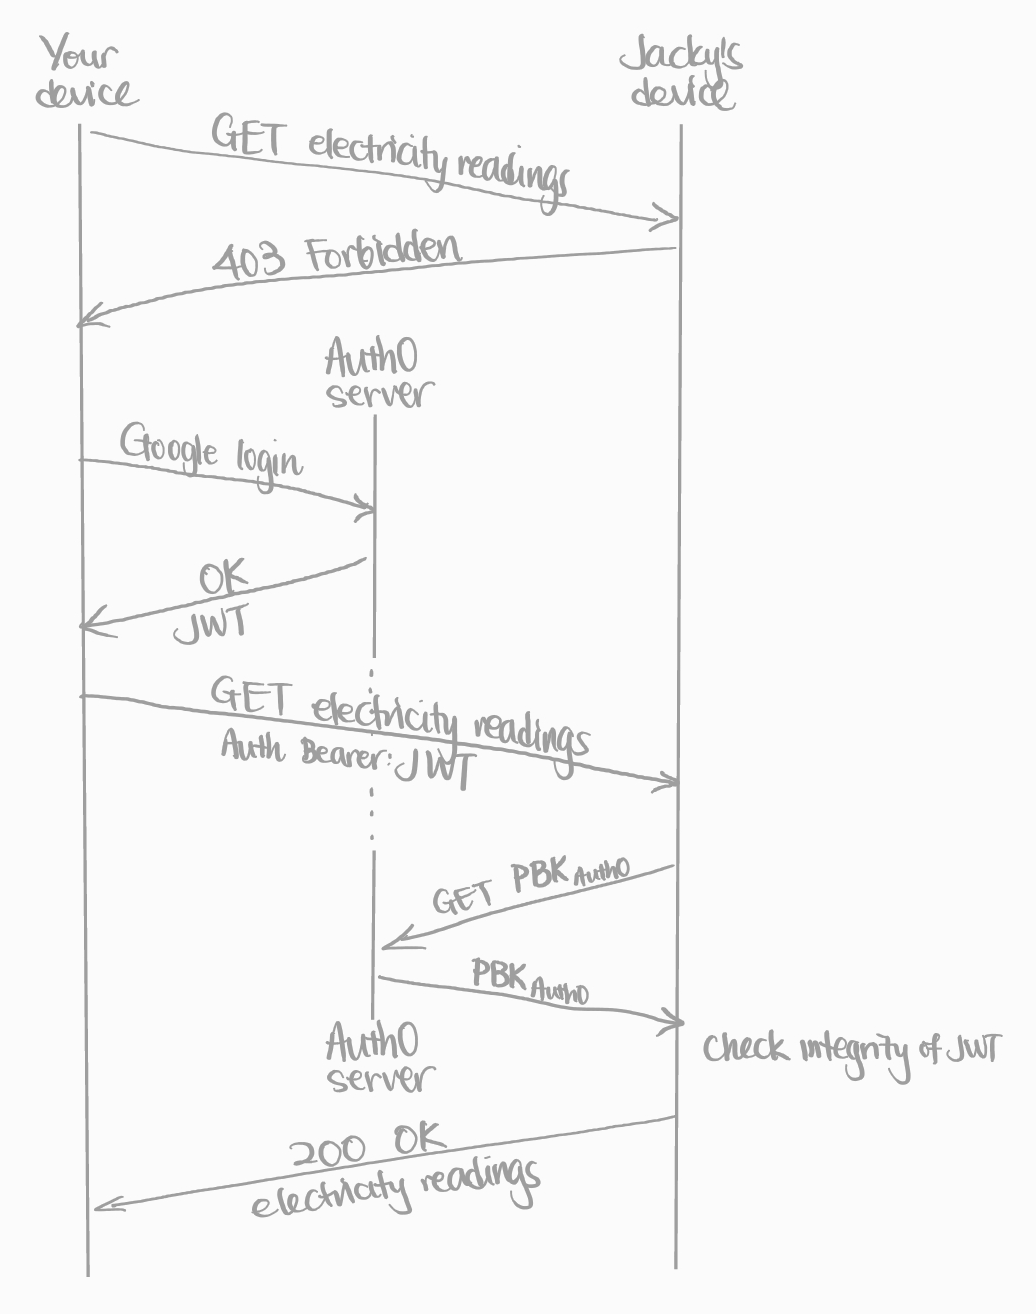
\includegraphics{Chapter 3 Client Auth.png}
    \caption{Outline of what happens before Jacky's device responds to each of your device's requests for data.}
    \label{clientauthflow}
\end{figure}

But Jacky's device is just a clueless server sitting on the Internet. How can it trust that the JWT you send over is legitimate (comes from \emph{Auth0})? After all, a JWT is just a (long) string of text, and your device can send anything it wants (with the help of some tools).

\newpage
\subsection{JSON Web Token (JWT) Structure}
A JWT is a (long) string of text that has this structure:
$$\text{encode}_{\text{base 64}}(\text{header})\ .\ \text{encode}_{\text{base 64}}(\text{payload})\ .\ \text{encode}_{\text{base 64}}(\text{signature})$$
Here's a screenshot from \href{https://jwt.io/}{jwt.io} that better illustrates this:

\begin{figure}[H]
    \centering
    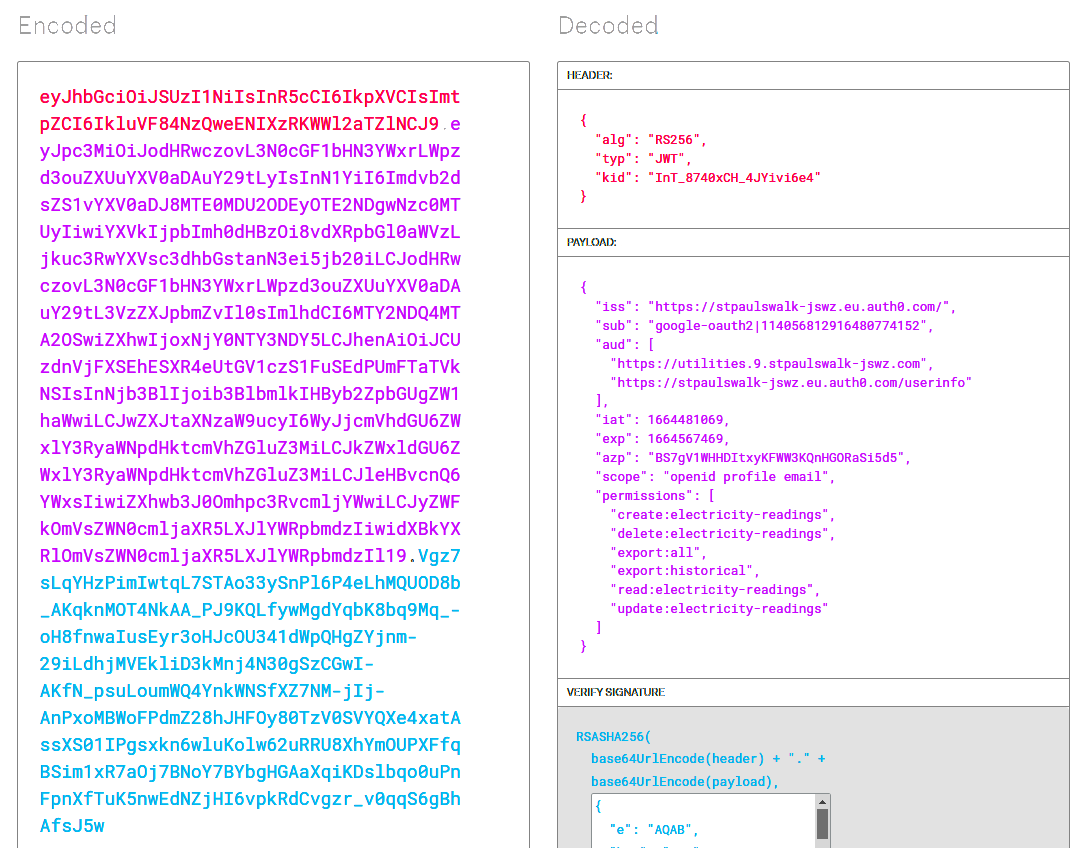
\includegraphics{Chapter 3 JWT.png}
    \caption{Internal structure of a JWT, illustrated by the JWT debugger \texttt{jwt.io}}
\end{figure}

What guarantees a JWT's legitimacy (that it comes from \emph{Auth0} and not anybody else) is its signature. Identically to how a signature works in Server Authenticity, the signature part of a JWT can only be generated by \emph{Auth0} using Auth0's private key $PVK_{Auth0}$.
$$\text{signature} = \text{encrypt}_{PVK_{Auth0}}\left(\text{hash}\Big(\text{encode}_{\text{base 64}}(\text{header})\ .\ \text{encode}_{\text{base 64}}(\text{payload})\Big)\right)$$
The above structure of the JWT signature is true for all JWTs: it's a standard.

\subsection{JWT Verification}
When receiving a JWT from your device, Jacky's device will do the following computation:
\begin{enumerate}[label=\arabic*.]
    \item From the JWT, obtain the first two sections:
    $$\text{encode}_{\text{base 64}}(\text{header})\ .\ \text{encode}_{\text{base 64}}(\text{payload})$$
    \item Hash the above value:
    $$\text{hash}\left(\text{encode}_{\text{base 64}}(\text{header}).\text{encode}_{\text{base 64}}(\text{payload})\right)$$
    \item From the JWT, obtain the encoded signature: $\text{encode}_{\text{base 64}}(\text{signature})$
    \item Decode the encoded signature to obtain the signature:
    \begin{align*}
        &\text{decode}_{\text{base 64}}\left(\text{encode}_{\text{base 64}}(\text{signature})\right) \\
        &= \text{signature} \\
        &= \text{encrypt}_{PVK_{Auth0}}\left(\text{hash}\Big(\text{encode}_{\text{base 64}}(\text{header})\ .\ \text{encode}_{\text{base 64}}(\text{payload})\Big)\right)
    \end{align*}
    \item Obtain \emph{Auth0}'s public key $PBK_{Auth0}$ by communicating directly with Auth0's server.
    \item Decrypt the signature: $$\text{decrypt}_{PBK_{Auth0}}\left(\text{encrypt}_{PVK_{Auth0}}\left(\text{hash}\Big(\text{encode}_{\text{base 64}}(\text{header})\ .\ \text{encode}_{\text{base 64}}(\text{payload})\Big)\right)\right)$$
    \item Test if the values from steps 2 and 6 are identical.
\end{enumerate}

If the test in step 7 fails, Jacky's device will reject the request for data. If it succeeds, then the JWT is 100\%\^{} guaranteed to originate from Auth0, and Jacky's device can trust the personal information that it contains. It then accepts the request and sends data back to your device.

Every JWT expires after a preset amount of time. This, and further details about what is in the $\text{payload}$ section of the JWT, will not be elaborated upon here, but are important for JWTs to provide client authenticity properly.

This concludes the Client Authenticity section. You now know how Jacky's device is able to trust your identity (vouched by \emph{Auth0}) when you make a request to it. In other words, we have client authenticity: Jacky's device knows it's talking to you.

\newpage
\section{Authorisation}
We only want the correct people to see our data. Authorisation is the operation of granting access to data only if the requester has sufficient permissions. Authorisation requires client authentication as a pre-requisite, which we already have as covered in the previous section.

Remember the JWT? Within the $\text{payload}$ section of the JWT, there is a permissions array. This is a list of the permissions that Jacky has granted you, via Auth0 (this is \emph{Auth0}'s \emph{Role-Based Access Control} feature).

When your device makes a request to Jacky's device, your device also sends along your JWT (see Figure \ref{clientauthflow}). Jacky's device will then inspect your JWT's permissions array, and send back data only if your permissions array contains what Jacky's device is looking for.

That's all there is to say for authorisation, no drawings here.

\subsection{Guarding against naughty users}
Suppose our favourite neighbour \chinese{隔壁老王} takes interest in our website and visits it. He obtains a JWT after logging in to Google via \emph{Auth0}. He wants to see everything. Can he modify his JWT and insert into the permissions array any permission that he likes?

No. \textlightgray{(Thank god!)}

Remember that the JWT contains a signature:
$$\text{signature} = \text{encrypt}_{PVK_{Auth0}}\left(\text{hash}\Big(\text{encode}_{\text{base 64}}(\text{header})\ .\ \text{encode}_{\text{base 64}}(\text{payload})\Big)\right)$$
This is encrypted using \emph{Auth0}'s private key $PVK_{Auth0}$. This encryption is an operation which \chinese{隔壁老王} most certainly cannot perform, because he does not possess $PVK_{Auth0}$: this is Auth0's secret!

The presence of the signature guards against malicious modifications to the JWT, and so this method of authorisation is secure.

\subsection{Importance of keeping secrets secret}
Of course, this security property of "only letting those with permissions see our data" breaks down if you share your JWT with third parties. Should they send your JWT along with their request for data, they will be able to gain access to our data, because to Jacky's device, it looks like \emph{you}, a legitimate user with sufficient permissions, are trying to access data.

Thus, it is crucial that you do not share your JWT with others. Same goes for the access tokens that you may see in the URLs of images and "Export Data" sections: the underlying concept is the same.

For ease of mind, the JWT is normally not visible when you use the website, it's handled automatically in the background by your browser.

This concludes the Authorisation section. You now know how Jacky's device is able to grant access to data only to people that are authorised to see our data. In other words, we have authorisation.

\end{document}
